\chapter{Διαδίκτυο των Πραγμάτων και εφαρμογές στην Βιοϊατρική}
\label{chap1}
\section{Διαδίκτυο των Πραγμάτων}
\subsection{Σκοπός}
Κατά τη διάρκεια της δεκαετίας 2010-2020, ο όρος Διαδίκτυο των Πραγμάτων (\en{Internet of Things} ή εν συντομία \en{IoT}) αποτέλεσε έναν ακόμη αναδυόμενο τεχνολογικό κλάδο, ο οποίος πέρασε από τα διάφορα στάδια αποδοχής και ωρίμανσης του (\en{Hype Cycle}), όπως αποδίδονται γραφικά στο Σχήμα \ref{hc}.
\begin{figure}[h!]
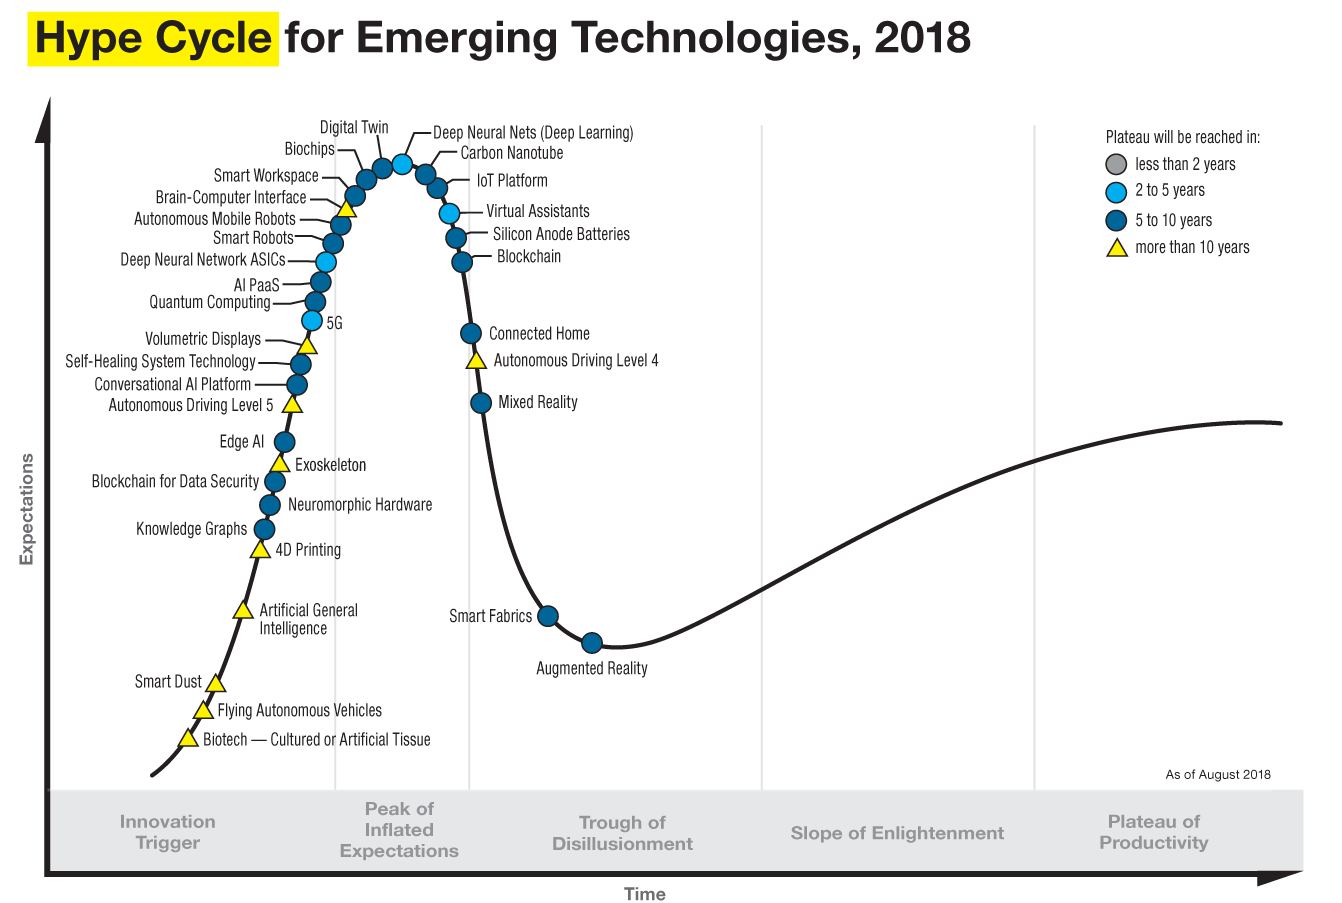
\includegraphics[scale=0.3]{images/hype_cycle.png}
\centering
\caption{Γραφική απεικόνιση της έννοιας του \en{Hype cycle} και απεικόνιση των διάφορων τεχνολογιών το 2018 από την \en{Gartner} \cite{Gartner:HC}}	
\label{hc}
\end{figure}
Λόγω του χάσματος μεταξύ των υψηλών προσδοκιών και των πραγματικών αποτελεσμάτων που έχει επιφέρει ο κλάδος, αλλά και λόγω της ασάφειας που χαρακτηρίζει πολλές σχετικές εφαρμογές, η ουσία και η πραγματική αξία του Διαδικτύου των Πραγμάτων δεν έχει αναδειχθεί επαρκώς στο ευρύ κοινό.
\par
Το Διαδίκτυο των Πραγμάτων είναι ένας τεχνολογικός κλάδος με αντικείμενο τη σχεδίαση και την υλοποίηση της μελλοντικής διεπαφής του φυσικού και του ψηφιακού χώρου.
Ο στόχος είναι η δημιουργία ενός περιβάλλοντος διάχυτης παρουσίας και παρακολούθησης, αποτελούμενο από διασυνδεδεμένα αντικείμενα, τα οποία αλληλεπιδρούν με το περιβάλλον τους και συνεργάζονται για την επίτευξη κοινών στόχων. \cite{book:giusto}
\par
Η επίτευξη αυτού του στόχου θα διαμορφώσει την καθημερινή ζωή και συμπεριφορά των ανθρώπων της εποχής, όπως ακριβώς το Διαδίκτυο συνεχίζει να μετασχηματίζει τις ζωές μας.
Ένα τέτοιο περιβάλλον θα επηρεάσει τομείς όπως η μετακίνηση ανθρώπων και αγαθών, ο αυτοματισμός, η βιομηχανική παραγωγή και τέλος ο τομέας της υγείας.
\par
Φυσικά, οι δυνατότητες αυτές δεν έχουν περάσει απαρατήρητες από τον επιχειρηματικό τομέα.
Συγκεκριμένα, οι εκτιμήσεις της \en{Cisco} προέβλεπαν ότι το 2022 θα υπάρχουν πάνω από 28.5 δισεκατομμύρια συνδεδεμένες συσκευές στο Διαδίκτυο \cite{cisco2019}, όπως αποδίδεται στο Σχήμα \ref{iotnumb}. Σύμφωνα με τα πραγματικά δεδομένα, η ανάπτυξη παρουσίασε ταχύτερους ρυθμούς από τις προβλέψεις.
Παράλληλα, η \en{Gartner, Inc.} εκτιμά ότι το 2020 περισσότερες από τις μισές νέες επιχειρησιακές διαδικασίες και συστήματα θα ενσωματώνουν κάποιο στοιχείο του \en{IoT} \cite{gartner2016}.
Τέλος, η \en{McKinsey} εκτιμούσε ότι το 2025 η οικονομική επίπτωση του κλάδου στην παγκόσμια οικονομία θα φτάσει τα τρισεκατομμύρια δολάρια \cite{mck2016}, προβλέψεις που έχουν επιβεβαιωθεί σε μεγάλο βαθμό.

\begin{figure}[h!]
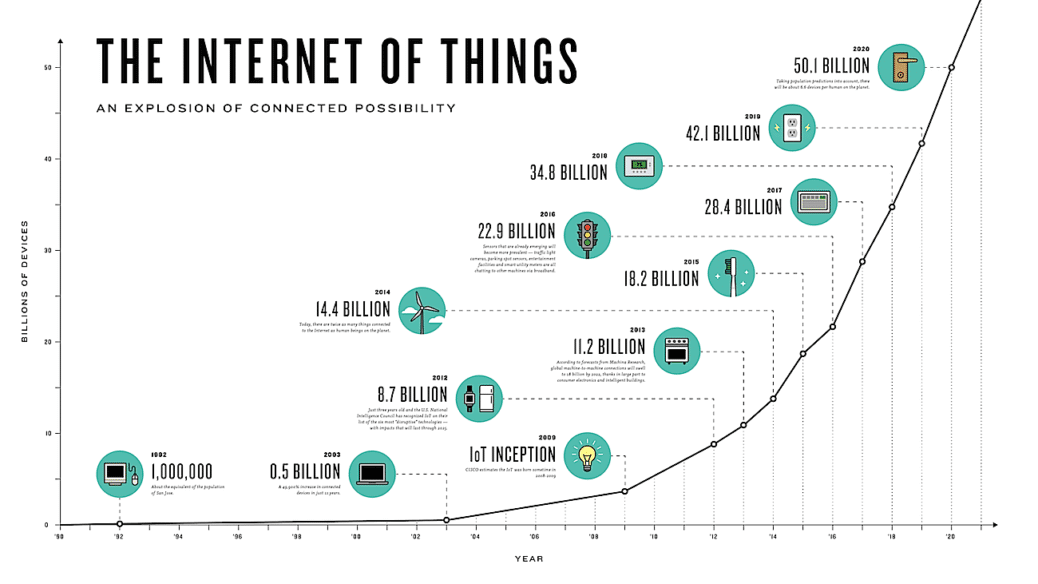
\includegraphics[scale=0.4]{images/IOT_numbes.png}
\centering
\caption{Γραφική απεικόνιση της εξέλιξης του αριθμού των συνδεδεμένων συσκευών στο Διαδίκτυο \cite{iotnumb}}	
\label{iotnumb}
\end{figure}

\subsection{Εισαγωγή}
Το \en{IoT} ορίζεται ως ``ένα παγκόσμιας εμβέλειας δίκτυο από άμεσα προσπελάσιμα, μοναδικά διευθυνσιοδοτημένα, διασυνδεδεμένα αντικείμενα, βασισμένο σε σαφώς ορισμένα πρωτόκολλα επικοινωνίας`` \cite{ATZORI20102787}.
Ουσιαστικά, αποτελεί μια επέκταση του Διαδικτύου, η οποία καθιστά εφικτή τη συνδεσιμότητα φυσικών αντικείμενων.
Η επαύξηση των δυνατοτήτων των αντικείμενων ή ``πραγμάτων``, επιτυγχάνεται με την ενσωμάτωση ηλεκτρονικών συστημάτων και αισθητήρων, τα οποία επιτρέπουν την επικοινωνία και αλληλεπίδραση με άλλα αντικείμενα μέσω του Διαδικτύου, καθώς και τον απομακρυσμένο έλεγχό και την παρακολούθησή τους.
\par
Οι δυνατότητες αυτές είναι αποτέλεσμα της σύγκλισης πολλαπλών ετερογενών τεχνολογικών τομέων.
Αρχικά, η συνεχιζόμενη επιβεβαίωση του νόμου του \en{Moore} και οι εξελίξεις στη μικροηλεκτρονική, επιτρέπουν την μαζική παραγωγή μικρών, φθηνών, φορητών ηλεκτρονικών συσκευών και αισθητήρων κάθε είδους.
Παράλληλα, την τελευταία δεκαετία παρατηρήθηκε δραστική αλλαγή στον τρόπο πρόσβασης στο διαδίκτυο.
Πλέον, οι φορητές συσκευές είναι υπεύθυνες για το μεγαλύτερο μερίδιο διακίνησης δεδομένων μέσω του διαδικτύου, σε αντίθεση με την παραδοσιακή δίοδο των προσωπικών υπολογιστών \cite{cisco2019}.
\par
Ταυτόχρονα, η ανάπτυξη του \en{Cloud Computing} επιτρέπει την εύκολη και αποδοτική διαχείριση πολύπλοκων υπολογιστικών συστημάτων και ετερογενών ροών δεδομένων.
Αυτό καθιστά την κατανεμημένη επεξεργασία και αποθήκευση δεδομένων εφικτή και προτιμότερη, σε σχέση με τη συγκεντρωτική παραδοσιακή εκδοχή.
Χαρακτηριστικό παράδειγμα αποτελεί ο τεχνολογικός κλάδος του \en{Edge Computing}, ο οποίος σκοπεύει στην ανάλυση και επεξεργασία των δεδομένων στη συσκευή ή στο περιβάλλον, στα οποία αυτά συλλέχθηκαν.
Επίσης, οι εξελίξεις στον τομέα της Μηχανικής Μάθησης επιτρέπουν την αποδοτική και άμεση εξαγωγή πληροφορίας και αξίας από αυτόν τον μεγάλο όγκο δεδομένων.
\par
Τέλος, η προτεραιότητα που δίνεται στον κλάδο του \en{IoT} από τους ακαδημαϊκούς και επιχειρηματικούς κύκλους, οφείλεται στην ανάδειξη του Διαδικτύου ως του νέου πεδίου καινοτομίας.
Κατά την τελευταία δεκαετία, αναδείχθηκαν νέες επιχειρήσεις ενώ παλιότερες επανατοποθετήθηκαν στρατηγικά, αξιοποιώντας τις νέες τεχνολογικές δυνατότητες για να επιλύσουν παραδοσιακά προβλήματα (π.χ. \en{Uber, Airbnb, Amazon}, κτλπ.).
\subsection{Αρχιτεκτονική}
\begin{figure}[h!]
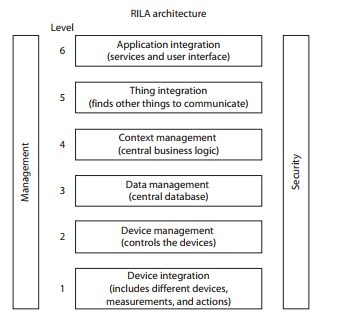
\includegraphics[scale=1.5]{images/iotrm3.png}
\centering
\caption{Γραφική απεικόνιση της πρότυπης αρχιτεκτονικής \en{IoT} εφαρμογών \cite{iotrm}}.
\label{iotrm}
\end{figure}
Έχουν γίνει πολλές προσπάθειες για να δημιουργηθούν πρότυπα μοντέλα και αρχιτεκτονικές για την ανάπτυξη εφαρμογών \en{IoT}.
Μια από τις κυρίαρχες αρχιτεκτονικές, η \en{RILA (Reference IoT Layered Architecture)}, αποδίδεται γραφικά στο Σχήμα \ref{iotrm}.
Η \en{RILA} αποτελείται από 6 οριζόντια και 2 κάθετα επίπεδα. Τα κάθετα επίπεδα αντιστοιχούν στη διαχείριση και την ασφάλεια, οι οποίες διατρέχουν όλα τα οριζόντια στρώματα της εφαρμογής.

Για την καλύτερη κατανόηση της αρχιτεκτονικής, παρατίθεται μια σύντομη περιγραφή κάθε επιπέδου. Να σημειωθεί πως αντικείμενο θεωρείται ένα οποιοδήποτε φυσικό αντικείμενο της καθημερινότητας μας, είτε πρόκειται για ένα ψυγείο, σπίτι ή ολόκληρη πόλη, ενώ συσκευή θεωρείται οποιοσδήποτε αισθητήρας ή ενεργοποιητής.
\begin{enumerate}
    \item \textbf{Ενσωμάτωση συσκευών} --- Αυτό το επίπεδο περιλαμβάνει την επικοινωνία με κάθε είδους συσκευή, αισθητήρα ή ενεργοποιητή, επικοινωνώντας με καθένα με το αντίστοιχο πρωτόκολλο, τον εντοπισμό ή διαγραφή νέων συσκευών, καθώς και την αδιάλειπτη επικοινωνία τους με τα ανώτερα στρώματα.
    \item \textbf{Διαχείριση συσκευών} --- Αυτό το επίπεδο ελέγχει τις συσκευές, καθώς έχει μια συνολική εικόνα του δικτύου. Συγκεκριμένα, περιλαμβάνει την εισαγωγή ή διαγραφή νέων συσκευών, την επικοινωνία των εντολών στους ενεργοποιητές, τον εμπλουτισμό των δεδομένων με \en{metadata} αναφορικά με το είδος του αισθητήρα από τον οποίο συλλέχθηκαν, και τέλος την προώθηση αυτών στα ανώτερα στρώματα.
    \item \textbf{Διαχείριση δεδομένων} --- Αυτό το επίπεδο μπορεί να θεωρηθεί η βάση δεδομένων της εφαρμογής, όπου τα δεδομένα που σχετίζονται με το αντικείμενο αποθηκεύονται.
    \item \textbf{Διαχείριση πλαισίου} --- Αυτό το επίπεδο ορίζει την λογική πίσω από την εφαρμογή και είναι υπεύθυνο για τα εξής:
        \begin{itemize}
            \item Ορίζει τους στόχους του αντικειμένου.
            \item Λαμβάνει και καταναλώνει το πλαίσιο άλλων αντικειμένων.
            \item Παράγει το πλαίσιο του αντικειμένου
            \item Αξιολογεί το πλαίσιο του σε σχέση με τους στόχους του.
            \item Προκαλεί ενέργειες προκειμένου να πετύχει τους στόχους του.
            \item Δημοσιεύει το πλαίσιο του για τα άλλα αντικείμενα
        \end{itemize}
    \item \textbf{Ενσωμάτωση αντικειμένων} --- Αυτό το επίπεδο είναι υπεύθυνο για τον εντοπισμό άλλων αντικειμένων και την επικοινωνία μαζί τους. Αφού 2 αντικείμενα έχουν βρεθεί, πρέπει να περάσουν μια διαδικασία εγγραφής, κατά την οποία συγκρίνονται τα σχήματα επικοινωνίας πλαισίου και ενεργειών. Αυτή η διαδικασία μπορεί να γίνει είτε κατανεμημένα είτε κεντρικά, σε ένα διαχειριστικό συστατικό. 
    \item \textbf{Ενσωμάτωση εφαρμογής} --- Αυτό το επίπεδο περιλαμβάνει την επικοινωνία του αντικειμένου με τον χρήστη, και η μορφή της καθώς και η υλοποίησή της εξαρτάται έντονα από την εφαρμογή.
\end{enumerate}
Όσον αφορά τα κάθετα επίπεδα, το πρώτο αναφέρεται στη διαχείριση του συστήματος, ενώ το δεύτερο στην ασφάλεια. Και τα δύο διασχίζουν όλα τα οριζόντια επίπεδα, καθώς ζητήματα διαχείρισης και ασφάλειας δεδομένων προκύπτουν σε κάθε στρώμα, από τα πρωτόκολλα επικοινωνίας των συσκευών μέχρι την λήψη αποφάσεων.

\subsection{Τεχνολογίες}
Όπως αναλύθηκε παραπάνω, το \en{IoT} περιλαμβάνει τεχνολογίες και έννοιες από πολλούς άλλους τομείς. Σε αυτό το σημείο, παρουσιάζονται οι ευρέως χρησιμοποιούμενες και σημαντικές τεχνολογίες, οι οποίες αποτελούν την βάση πολλών \en{IoT} εφαρμογών.
\subsubsection{\en{Radio frequency identification (RFID)}}
Η ταυτοποίησή ανθρώπων και αντικείμενων μέσα σε ένα κατανεμημένο δίκτυο αποτελεί βασική προϋπόθεση για οποιαδήποτε εφαρμογή \en{IoT}. Στις περισσότερες εφαρμογές χρησιμοποιούνται ετικέτες \en{RFID (RFID tags)}, οι οποίες επιτρέπουν την απόδοση ενός μοναδικού προσδιοριστικού σε όποιο αντικείμενο είναι ενσωματωμένα. Μια ετικέτα \en{RFID} είναι ένας μικρός επεξεργαστής, ο οποίος εκτελεί την στοιχειώδη λειτουργία του να μεταδίδει δεδομένα σε τυχόν ερωτήσεις από μια συσκευή ανάγνωσης (\en{RFID reader}).
\par
Υπάρχουν 3 ειδών ετικέτες \en{RFID}, ανάλογα με την πηγή ενέργεια τους.
Στην πρώτη κατηγορία ανήκουν οι ``παθητικές`` ετικέτες \en{RFID}, οι οποίες δεν περιέχουν κάποια πηγή ενέργειας, αλλά εκμεταλλεύονται την ενέργεια του λαμβανόμενου σήματος για να αποστείλουν τα απαραίτητα δεδομένα, όπως απεικονίζεται στο Σχήμα \ref{passRFID}.
Για αυτόν τον λόγο, συνήθως έχουν μικρό μέγεθος και χαμηλό κόστος.
\begin{figure}[h!]
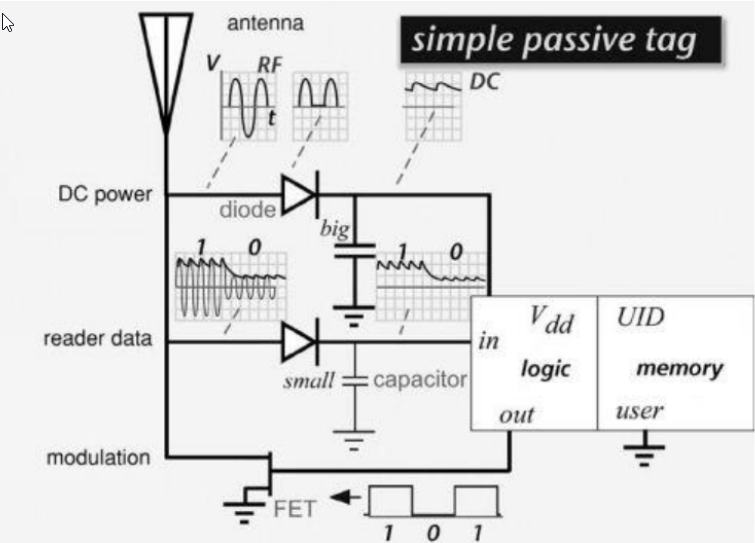
\includegraphics[scale=0.7]{images/pass_RFID.png}
\centering
\caption{Σχηματική απεικόνιση μιας ``παθητικής`` ετικέτας \en{RFID}\cite{rfidpass}.}
\label{passRFID}
\end{figure}
Στην δεύτερη κατηγορία ανήκουν οι ``ήμι-παθητικές`` ετικέτες, οι οποίες έχουν μπαταρία, αλλά την χρησιμοποιούν μόνο για την λειτουργία τους σε περίπτωση ερώτηση από συσκευή ανάγνωσης.
Τέλος, στην τρίτη κατηγορία ανήκουν οι ``ενεργητικές`` ετικέτες, οι οποίες έχουν μπαταρία και περιοδικά μεταδίδουν την πληροφορία τους και έτσι μπορούν να υποκινήσουν την επικοινωνία με μια συσκευή ανάγνωσης.
Προφανώς, οι ετικέτες που περιέχουν πηγή ενέργειας είναι μεγαλύτερες σε μέγεθος και έχουν υψηλότερο κόστος σε σχέση με τις ``παθητικές``.
\par
Οι ιδιότητες των συστημάτων \en{RFID}, που τα καθιστούν θεμέλιο λίθο του \en{IoT} είναι οι εξής:
\begin{itemize}
    \item \textbf{Μικρό μέγεθος} --- Οι μικρότερες ετικέτες \en{RFID} έχουν μέγεθος της τάξεως του 1\(mm^2\) \cite{smalltag}, οπότε υπάρχει η δυνατότητα ενσωμάτωσης σε κάθε είδους φυσικό αντικείμενο.
    Προφανώς, υπάρχει γραμμική σχέση μεταξύ του μεγέθους και της εμβέλειας της ετικέτας, οπότε η επιλογή της ετικέτας εξαρτάται από το είδος της εφαρμογής.
    \item \textbf{Χαμηλό κόστος} --- Οι φθηνότερες ετικέτες \en{RFID} κοστίζουν λιγότερο από 0.10€.
    \item \textbf{Μοναδικός τρόπος ανίχνευσης} --- Οι ετικέτες \en{RFID} εκπέμπουν έναν μοναδικό σειριακό αριθμό, οπότε επιτρέπουν την ταυτοποίηση ενός αντικείμενου από άλλα παρόμοια αντικείμενα.
    \item \textbf{Αυτοματοποίηση} --- Η διαδικασία ταυτοποίησης γίνεται αυτόματα από την συσκευή ανάγνωσης. Ενδεικτικά, μια συσκευή ανάγνωσης μπορεί να διαβάσει μέχρι και 300 ετικέτες το δευτερόλεπτο \cite{rainrfid}.
\end{itemize}

\subsubsection{Πρωτόκολλα επικοινωνίας}
Όπως είναι σαφές από την αρχιτεκτονική της, μια εφαρμογή \en{IoT} στηρίζεται στην επικοινωνία μεταξύ πολλών, ετερογενών οντοτήτων.
Το λογισμικό, το οποίο φροντίζει για την τήρηση αυτών των πρωτοκόλλων, ονομάζεται \en{middleware}.
Η αφαίρεση αυτής της πολύπλοκης διαδικασίας επιτρέπει την γρήγορη ανάπτυξη νέων εφαρμογών και την αντίστοιχα γρήγορη ενσωμάτωση παλαιότερων.
Το \en{RFC 7452} \cite{rfc7452} συνοψίζει 4 πρότυπα επικοινωνίας που χρησιμοποιούνται σε \en{IoT} εφαρμογές.
\begin{itemize}
    \item \textbf{\en{Device-to-device}} --- Πρόκειται για την περίπτωση άμεσης επικοινωνίας 2 συσκευών, συνήθως ασύρματα.
    Ανάλογα με την εφαρμογή και τις συσκευές, χρησιμοποιούνται άλλα πρωτόκολλα.
    Αυτά περιλαμβάνουν το \en{Bluetooth} ή \en{6LoWPAN}, \en{IPv6}, \en{UDP} και \en{CoAP}.
    \item \textbf{\en{Device-to-cloud}} --- Πρόκειται για την περίπτωση μεταφοράς δεδομένων από την συσκευή σε ένα σύστημα επεξεργασίας και αποθήκευσης, συνήθως στο \en{Cloud}. Η επικοινωνία βασίζεται στο \en{IP}.
    \item \textbf{\en{Device-to-gateway}} --- Πρόκειται για την περίπτωση στις οποίες το σύστημα περιλαμβάνει συσκευές που δεν μπορούν να συνδεθούν άμεσα στο Διαδίκτυο. Σε αυτές τις περιπτώσεις χρησιμοποιείται ένας εξυπηρετητής, ο οποίος παρεμβάλλεται μεταξύ των συσκευών και του Διαδικτύου. Ο εξυπηρετητής αυτός θα πρέπει να είναι σε θέση να επικοινωνεί με τις συγκεκριμένες συσκευές.
    \item \textbf{\en{Backend data sharing}} --- Πρόκειται για την περίπτωση μεταφοράς δεδομένων για να γίνει κεντρική ανάλυση. Αυτή η περίπτωση περιλαμβάνει την μεταφορά δεδομένων μεταξύ εφαρμογών \en{IoT}.
\end{itemize}
\par
Στον Πίνακα \ref{iotcomm} αναφέρονται μερικές από τις πιο διαδεδομένες τεχνολογίες επικοινωνίας και τα χαρακτηριστικά τους.
\begin{table}[h!]
    \footnotesize
    \centering
    \begin{tabularx}{\textwidth}{>{\hsize=.4\hsize}X >{\hsize=.75\hsize}X >{\hsize=.7\hsize}X X}
        Όνομα&Συχνότητα&Εμβέλεια&Εφαρμογές
        \\
        \hline
        \en{BLE}&2.4 \en{GHz}&1-100 μ.& Ακουστικά, \en{wearables}, εφαρμογές υγείας, εφαρμογές αυτοβιομηχανίας, αισθητήρες εγγύτητας, κτλπ.
         \\
         \en{EnOcean}&315, 868, 902 \en{MHz}&\(>100\) μ.& Παρακολούθηση και έλεγχος συστημάτων και αυτοματισμών, μεταφορές και \en{logistics}
         \\
         \en{GSM}&900 \en{MHz} και 1.8 \en{GHz}&30 - 300 μ.& Κινητά τηλέφωνα, παρακολούθηση στόχων, M2M
         \\
         \en{LoRa}& \(< 1\) \en{GHz ISM} μπάντα&2-45 χλμ. (ανάλογα με το περιβάλλον)& Εφαρμογές μακριάς εμβέλειας, μητροπολιτικές, M2M
         \\
         \en{NB-IoT}&700-900 \en{MHz}&10-15 χμ.& Βιομηχανική παρακολούθηση, ``έξυπνα`` σπίτια, ``έξυπνες`` πόλεις, ανίχνευση γεγονότων
         \\
         \en{NFC}& 13.56 \en{MHz}& \(< 0.2\) μ. & Διαχείριση πρόσβασης, ``έξυπνες`` κάρτες, ``έξυπνα`` πορτοφόλια
         \\
         \en{NWave}& \(< 1\) \en{GHz ISM} μπάντα&\(< 10\) χλμ.& Γεωργικές και περιβαλλοντικές εφαρμογές, εφοδιαστική αλυσίδα, ``έξυπνες`` πόλεις
         \\
         \en{RFID}& 120-150 \en{kHz (LF)}, 13.56 \en{MHz (HF)}, 865-868 \en{MHz (UHF)}, 2.4-10 \en{GHz} (μικροκύματα) &10 εκ. - 200 μ.& Διόδια, εφοδιαστική αλυσίδα, παρακολούθηση και καταγραφή αγαθών, διαχείριση πρόσβασης
         \\
        \en{SigFox}&900 \en{MHz}&3-50 χλμ. (ανάλογα με το περιβάλλον)& Εφαρμογές ασφαλείας και απομακρυσμένης παρακολούθησης
         \\
        \en{Weightless}&470-790 \en{MHz}&\(< 10\) χλμ.& Βιομηχανική παρακολούθηση, αισθητήρες κίνησης
         \\
        \en{Wi-Fi}&2.4 \en{GHz}, 3.6 \en{GHz}, 4.9/5 \en{GHz}&\(< 100\) μ.& Διακομιστές, κινητά τηλέφωνα, προσωπικοί υπολογιστές
         \\
        \en{Z-Wave}&865-926 \en{MHz}&100 μ.& Παρακολούθηση και έλεγχος ``έξυπνων`` σπιτιών και εμπορικών καταστημάτων
        \\
        \en{ZigBee}&868 \en{MHz}, 2.4 \en{GHz}&10-20 μ.& βιομηχανικός έλεγος, αυτοματισμοί σπιτιών και κατασκευών, \en{WSN}
    \end{tabularx}
    \caption{Δημοφιλή πρωτόκολλα επικοινωνίας}
    \label{iotcomm}
\end{table}

\subsubsection{\en{Cloud Computing}}

Οι \en{IoT} εφαρμογές απαιτούν επεξεργασία και αποθήκευση ετερογενών και μη σταθερών ροών δεδομένων.
Αυτήν, ακριβώς, την ανάγκη καλύπτει ο κλάδος του \en{Cloud computing}, ο οποίος παρέχει πρόσβαση σε υπολογιστικές υποδομές ή λογισμικό, τα οποία προσαρμόζονται ανάλογα με τις ανάγκες και την ζήτηση.
\par
Σύμφωνα με αρκετές οπτικές \cite{iotcloud1}\cite{iotcloud2}, τα 2 πεδία είναι συμπληρωματικά, καθώς οι \en{IoT} εφαρμογές προσφέρουν την κατανεμημένη παρουσία και τα δεδομένα από το φυσικό περιβάλλον, ενώ οι \en{Cloud} εφαρμογές προσφέρουν τους πόρους και τις υπηρεσίες που υπολείπονται οι \en{IoT} συσκευές.
Συγκεκριμένα, οι υπηρεσίες που προσφέρει το \en{Cloud} ομαδοποιούνται σε 3 κατηγορίες.
\begin{itemize}
    \item \textbf{Επικοινωνία} --- Το \en{Cloud} καθιστά δυνατή και φθηνή, την σύνδεση, παρακολούθηση και διαχείριση αντικειμένων εξ αποστάσεως, καθώς και την αυτοματοποίηση αυτών των διαδικασιών.
    \item \textbf{Αποθήκευση} --- Το \en{Cloud} καθιστά δυνατή και φθηνή, την συλλογή, αποθήκευση, συσσωμάτωση, ενσωμάτωση και, τέλος, την ομογενοποίηση των ετερογενών ροών δεδομένων, τα οποία παράγουν τα διάφορα αντικείμενα.
    \item \textbf{Επεξεργασία} --- Το \en{Cloud} καθιστά δυνατή την κεντρική, σύγχρονη και επεκτάσιμη επεξεργασία, η οποία είναι αδύνατη με τους περιορισμούς πόρους των \en{IoT} συσκευών.
\end{itemize}
\par

\subsection{Προκλήσεις}
Το \en{IoT}, ωστόσο, είναι ένας απότομα αναδυόμενος τομέας.
Οι υποδομές και, κυρίως, οι διαδικασίες που το συνθέτουν είναι ακόμα υπό διαμόρφωση.
Η πρώτη δεκαετία ανάπτυξης και εδραίωσης του \en{IoT} ανέδειξε κρίσιμα ερωτήματα και προβληματισμούς για το μέλλον του, μερικοί από τους οποίους αναφέρονται παρακάτω.
\subsubsection{Ασφάλεια}
Σαν δομικό στοιχείο κάθε δικτύου, η ασφάλεια αποτελεί ένα από τα μεγαλύτερα εμπόδια για την πλήρη ανάπτυξη του \en{IoT} \cite{foster}.
Η αλματώδης αύξηση του αριθμού και της ποικιλίας των, συνδεδεμένων στο διαδίκτυο, συσκευών αυξάνει τις πιθανές απειλές στην ασφάλεια των χρηστών.

Λόγω της έμφυτης ετερογένειας του \en{IoT}, δεν υπάρχει μια τυποποιημένη λύση για την ασφάλεια των εφαρμογών του, αλλά ορισμένοι κοινοί στόχοι.
\begin{itemize}
    \item \textbf{Εμπιστευτικότητα} --- Η πρόσβαση σε δεδομένα θα γίνεται μόνο από εξουσιοδοτημένα άτομα. Η εμπιστευτικότητα των δεδομένων είναι ιδιαίτερα σημαντική στις εφαρμογές που διαχειρίζονται ευαίσθητα προσωπικά δεδομένα.
    \item \textbf{Ακεραιότητα} --- Μια \en{IoT} εφαρμογή ή συσκευή πρέπει να διατηρεί την ακρίβεια, την συνέπεια και την αξιοπιστία των δεδομένων που αποθηκεύουν ή διαχειρίζονται. Πολύ συχνά, οι \en{IoT} συσκευές περιέχουν ευαίσθητα δεδομένα, και οποιαδήποτε μη εξουσιοδοτημένη αλλαγή σε αυτά μπορεί να έχει τεράστιες επιπτώσεις στους χρήστες.
    \item \textbf{Διαθεσιμότητα} --- Ένα \en{IoT} σύστημα ή υπηρεσία οφείλει να είναι διαθέσιμη στους εξουσιοδοτημένους χρήστες. Επιπλέον, οι χρήστες αυτοί πρέπει να έχουν πρόσβαση στα δεδομένα που τους αντιστοιχούν. Οι \en{IoT} εφαρμογές, οφείλουν να προστατεύουν τα δεδομένα και τα συστήματα τους είτε από κακόβουλες ενέργειες είτε απο αστοχίες υλικού ή λογισμικού.
\end{itemize}
\subsubsection{Δια-λειτουργικότητα}
Ήδη, έχουμε μιλήσει αρκετά για τα διάφορα προβλήματα που προκαλεί ο υψηλός βαθμός ετερογένειας που εμφανίζει το \en{IoT}.
Η ανάπτυξη μιας εφαρμογής \en{IoT} απαιτεί την διαχείριση ενός έντονα δυναμικού κατανεμημένου συστήματος, το οποίο αποτελείται από πολλές και ποικίλες συσκευές.
Η χρήση και εδραίωση μιας πρότυπης \en{IoT} αρχιτεκτονικής θα επιτρέψει την κανονικοποιήση της διαδικασίας ανάπτυξης εφαρμογών, ενώ ο περαιτέρω έλεγχος και ανάπτυξη των απαραίτητων πρωτοκόλλων επικοινωνίας θα απλοποιήσει τα ζητήματα συνδεσιμότητας των συσκευών.
\subsubsection{Επεκτασιμότητα και αξιοποίηση δεδομένων}
Καθώς το δίκτυο των διασυνδεδεμένων συσκευών θα μεγαλώνει, οι απαιτήσεις από τις υποδομές θα αυξάνονται επίσης.
Ενώ τα ζητήματα επεκτασιμότητας του δικτύου θεωρούνται διαχειρίσιμα \cite{borgia2014}, δεν ισχύει το ίδιο για τις υποδομές που διαχειρίζονται δεδομένα.
Το μέγεθος των παραγόμενων δεδομένων δεν επιτρέπει την αποθήκευση τους σε μια κεντρική βάση δεδομένων, ενώ η μεταφορά τους απαιτεί απαγορευτικές ποσότητες υπολογιστικών πόρων.
Η λύση σε αυτά τα προβλήματα απαιτεί την χρήση και την ανάπτυξη νέων \en{Cloud} εφαρμογών, που θα επιτρέπουν την κατανεμημένη αποθήκευση και επεξεργασία δεδομένων.
Πέρα από την διαχείριση των δεδομένων, προκύπτει και το ζήτημα της αξιοποίησης τους.
Η χρήση και η ανάπτυξη νέων τεχνικών εξόρυξης δεδομένων γίνεται απαραίτητη, λόγω του μεγέθους και της έλλειψης δομής των δεδομένων.
\subsubsection{Αξιοποίηση των δυνατοτήτων του \en{IoT}}
Η εξέλιξη και η ανάπτυξη των προϊόντων και των τεχνολογιών, που απαρτίζουν το \en{IoT}, κινούνται με πολύ γρήγορο ρυθμό, συγκριτικά με άλλους κλάδους. 
Αυτό συμβαίνει καθώς το \en{IoT} αποτελεί ένα προσοδοφόρο έδαφος για την ανάπτυξη νέων προϊόντων μαζικής παραγωγής αλλά και νέων επιχειρηματικών τομέων, με μεγάλο περιθώριο κέρδους. 
Αυτό οδηγεί στην ανάπτυξη μεγάλου πλήθους προϊόντων, τα οποία δεν είναι επαρκώς ελεγμένα, και είναι διάτρητα από την οπτική της ασφάλειας και της ιδωτικότητας. 
Ταυτόχρονα, αναπτύσσονται ανταγωνιστικά μοντέλα και πρότυπα επικοινωνίας και ανάπτυξης εφαρμογών, τα οποία καθιστούν το \en{IoT} ιδιαίτερα κλειστό, με τις εφαρμογές του να είναι ελάχιστα επεκτάσιμες ή επαναχρησιμοποιήσιμες. 
\subsection{Εφαρμογές}
Όπως είναι σαφές από τα παραπάνω, το \en{IoT} μπορεί να εφαρμοστεί σε πολλούς υπάρχοντες κλάδους, με σκοπό την επέκταση των δυνατοτήτων τους και τη σύνδεσή τους με τον ψηφιακό κόσμο.
Επίσης, επιτρέπει τη μείωση του κόστους και την αύξηση της ποιότητας και της αξιοπιστίας των παρεχομένων υπηρεσιών. 
Ωστόσο, η ανάπτυξη του \en{IoT}, κυρίως, θα παράξει νέους τομείς και υπηρεσίες.
\par
Παρακάτω, παρατίθενται οι τομείς και οι εφαρμογές, οι οποίοι θα επηρεαστούν περισσότερο από την ανάπτυξη του \en{IoT}, καθώς και μια σχηματική απεικόνιση της διείσδυσης του \en{IoT} στη καθημερινότητα (Σχήμα \ref{iotapp}).
\begin{figure}[h!]
\centering
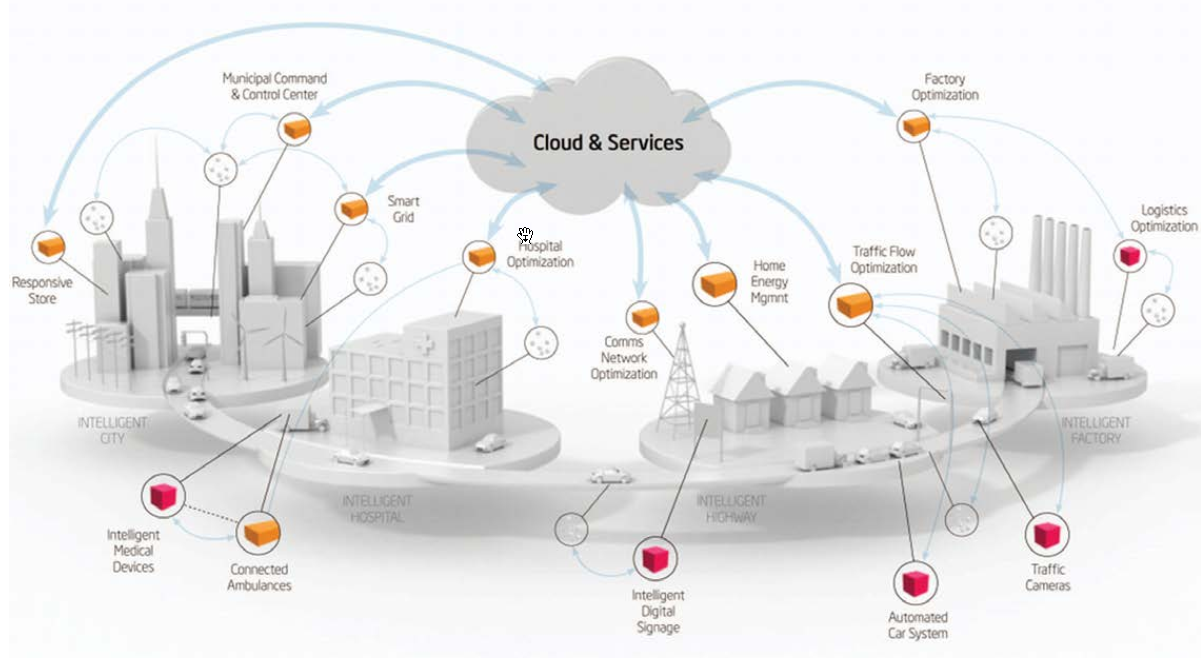
\includegraphics[scale=0.6]{images/iot_applications.png}
\caption{Σχηματική απεικόνιση των εφαρμογών του \en{IoT} \cite{iot_applications}}.
\label{iotapp}
\end{figure}

\subsubsection{Βιοϊατρική}
Οι εφαρμογές του \en{IoT} στον τομέα της Υγείας είναι πολλές και ποικίλες και αποτελούν το κύριο θέμα αυτής της διπλωματικής εργασίας. Θα αναφερθούμε εκτενέστερα στην ενότητα \ref{biomed} για τις εφαρμογές του \en{IoT} στον συγκεκριμένο τομέα.
\subsubsection{Μεταφορές και εφοδιαστική αλυσίδα}
Η χρήση αισθητήρων, ενεργοποιητών και επεξεργαστών επιτρέπει τον πιο ακριβή έλεγχο και χειρισμό των μεταφορικών μέσων, των μεταφερόμενων αγαθών, αλλά και της αντίστοιχης υποδομής, όπως οι δρόμοι, οι σταθερές τροχιές και οι αποθήκες διαχείρισης αγαθών.
Παρακάτω, αναφέρονται συγκεκριμένες εφαρμογές του \en{IoT} στον τομέα.
\begin{itemize}
    \item \textbf{Εφοδιαστική αλυσίδα} --- Η χρήση τεχνολογιών \en{RFID} και \en{NFC} επιτρέπουν την παρακολούθηση σε πραγματικό χρόνο κάθε κρίκου της εφοδιαστικής αλυσίδας, από τον σχεδιασμό των εμπορευμάτων και την παραγωγή μέχρι την διανομή και πώληση των προϊόντων.
    Αυτό, οδηγεί, στην ευελιξία της εφοδιαστικής αλυσίδας και την δυνατότητα προσαρμογής της σε πολύπλοκες και δυναμικές αγορές.
    \item \textbf{Υποβοηθούμενη οδήγηση} --- Εφαρμογές \en{IoT} μπορούν να παρέχουν πληροφορίες στους οδηγούς και επιβάτες των οχημάτων για καλύτερη πλοήγηση και ασφάλεια. Χαρακτηριστικές εφαρμογές είναι η διαχείριση της κυκλοφορίας των οχημάτων στους δρόμους, είτε αφορά σχεδιαστικούς σκοπούς είτε αφορά την πιο ασφαλή και γρήγορη πλοήγηση εμπορευμάτων.
    \item \textbf{Παρακολούθηση περιβαλλοντολογικών δεικτών} --- Η ασφαλής μεταφορά τροφίμων απαιτεί την τήρηση αυστηρών κανονισμών για την διατήρηση της ποιότητας τους.
    Συνήθως, αυτοί απαιτούν τις συνθήκες συντήρησης των τροφίμων να είναι συγκεκριμένες, με αυστηρά όρια στην θερμοκρασία και στην υγρασία του χώρου μεταφοράς. Η χρήση αισθητήρων επιτρέπουν την απρόσκοπτη παρακολούθηση των συνθηκών μεταφοράς τροφίμων.
\end{itemize}

\subsubsection{Έξυπνα περιβάλλοντα}
Ένα "έξυπνο περιβάλλον" είναι σε θέση να λαμβάνει πληροφορίες και να ενεργεί ανάλογα με αυτές, μέσω των αντικειμένων που το αποτελούν, διευκολύνοντας τους χρήστες του να επιτύχουν τους σκοπούς τους. Αυτός ο ορισμός περιλαμβάνει πολλές και ποικίλες χρήσεις, κάποιες από τις οποίες αναφέρονται παρακάτω. 
\begin{itemize}
    \item \textbf{Κατοικία και εργασιακοί χώροι} --- Η χρήση των δυνατοτήτων του \en{IoT} είναι σε θέση να μειώσει το κόστος και το περιβαλλοντολογικό αντίκτυπο της οικιστικής και επαγγελματικής χρήσης των κτηρίων\cite{iothome}. Ταυτόχρονα, η αυτοματοποίηση των διαδικασιών ελέγχου και παρακολούθησης, οδηγεί στην βελτίωση των συνθηκών ασφαλείας καθώς και την πιο άνετη διαβίωση των κατοίκων/υπαλλήλων.
    \item \textbf{Βιομηχανική και αγροτική παραγωγή} --- Οι εφαρμογές \en{IoT}, ήδη, διαδραματίζουν μεγάλο ρόλο στην βιομηχανία \cite{iotmanuf} και στην γεωργία \cite{iotagric}, καθώς καθιστούν δυνατή την περαιτέρω αυτοματοποίηση της παραγωγής.
    Συγκεκριμένα, στην βιομηχανική παραγωγή, οι δυνατότητες του \en{IoT} επιτρέπουν την βελτιστοποίηση της παραγωγής, τον άμεσο εντοπισμό και διόρθωση σφαλμάτων καθώς και την διαχείριση του εργασιακού περιβάλλοντος.
    Ταυτόχρονα, στην αγροτική παραγωγή, επιτρέπουν τον έλεγχο της άρδευσης, την παρακολούθηση των περιβαλλοντικών συνθηκών, των εντόμων και των άλλων ζώων που επηρεάζουν την παραγωγή.
    \item \textbf{Πόλεις} --- Η χρήση των δυνατοτήτων του \en{IoT} επιτρέπει, πλέον, την παρακολούθηση των υπηρεσιών και των συνθηκών μιας πόλης σε πραγματικό χρόνο.
    Αυτές ποικίλουν από την διαχείριση της κυκλοφορίας των οχημάτων μέχρι την διαχείριση κοινωφελών αγαθών, όπως η συγκομιδή απορριμάτων και η ύδρευση.
    Ιδιαίτερο ενδιαφέρον, παρουσιάζουν οι εφαρμογές που σχετίζονται με το \en{CIM (City Information Model)} \cite{iotcity}.
    Πρόκειται για την ιδέα ενός αστικού ιστού, πλήρως διασυνδεδεμένου, που επιτρέπει την παρακολούθηση και έλεγχο κάθε συστατικού του στοιχείου, είτε αυτό πρόκειται για κτήρια είτε πρόκειται για υποδομές, όπως το ηλεκτρικό δίκτυο.
\end{itemize}
\begin{comment}{}
\section{Μηχανική Μάθηση}
\subsection{Εισαγωγή}
Την τελευταία δεκαετία, η Μηχανική Μάθηση, όπως το \en{Internet of Things}, αποτέλεσε έναν τεχνολογικό κλάδο με εκρηκτική ανάπτυξη και δυσανάλογα υψηλές προσδοκίες.
Η Μηχανική Μάθηση είναι ένα υπολογιστικό πεδίο της Τεχνητής Νοημοσύνης. 
Αντικείμενο του είναι η κατασκευή συστημάτων αυτόματης μάθησης και βελτιστοποίησης, χωρίς σαφείς κανόνες για τον υπολογισμό ή την λύση προβλημάτων.
Στην βάση της μηχανικής μάθησης υπάρχει η υπόθεση ότι \textit{η γνώση μπορεί να προκύψει από τα δεδομένα.}
\par
Οι αλγόριθμοι μηχανικής μάθησης βασίζονται σε ένα σύνολο δεδομένων εισόδου, το οποίο ονομάζεται σύνολο εκπαίδευσης.
Αυτό αποτελείται από παραδείγματα της εισόδου του τελικού συστήματος ή εμπειρικά αποτελέσματα του συστήματος προς προσομοίωση.
Το σύνολο εκπαίδευσης χρησιμοποιείται για την αναγνώριση επαναλαμβανόμενων προτύπων στα δεδομένα και να οδηγήσει σε καλύτερες αποφάσεις στο μέλλον.
\par
Οι αλγόριθμοι μηχανικής μάθησης διακρίνονται σε 2 κατηγορίες, με κριτήριο τον τρόπο μάθησης, δηλαδή το πως δίνεται ανάδραση στο αναπτυσσόμενο σύστημα.
Δύο από τις ευρέως υιοθετούμενες μεθόδους μηχανικής μάθησης είναι η \textit{επιβλεπόμενη μάθηση} και η \textit{μη επιβλεπόμενη μάθηση}.
Η πρώτη απαιτεί την επισήμανση των παρατηρήσεων του συνόλου εκπαίδευσης με το επιθυμητό αποτέλεσμα του τελικού συστήματος, ενώ η δεύτερη δεν χρειάζεται την πληροφορία αυτή.
\subsection{Επιβλεπόμενη μάθηση}
Η επιβλεπόμενη μάθηση χρησιμοποιείται για την εκμάθηση της συνάρτησης απεικόνισης \(f\) από μερικές μεταβλητές εισόδου \(X\) σε μια μεταβλητή εξόδου \(Y\).
\begin{equation}
  Y = f(X)  
\end{equation}
Ο σκοπός της επιβλεπόμενης μάθησης είναι να προσεγγίσει την δομή της συνάρτησης απεικόνισης, έτσι ώστε να μπορεί να γενικεύσει και να προβλέπει σωστά το αποτέλεσμα καινούργιων παρατηρήσεων. 
Η διαδικασία μάθησης περιλαμβάνει την επαναλαμβανόμενη πρόβλεψη των αποτελεσμάτων των δεδομένων εισόδου, την σύγκριση με τις γνωστές, σωστές απαντήσεις και την διόρθωση των παραμέτρων του εκάστοτε μοντέλου.
Η διαδικασία αυτή σταματά όταν επιτευχθεί κάποιο κριτήριο, το οποίο συνήθως είναι αριθμός επαναλήψεων ή κάποιο κριτήριο απόδοσης.
Η χρήση επιβλεπόμενης μάθησης χρησιμοποιείται συνήθως σε προβλήματα \textit{παλινδρόμησης \en{(regression)}} και σε προβλήματα  \textit{ταξινόμησης \en{(classification)}}.
Η μεταβλητή εξόδου στα προβλήματα παλινδρόμησης είναι συνεχής, ενώ, αντίθετα, στα προβλήματα ταξινόμησης είναι διακριτή.
\subsection{Μη επιβλεπόμενη μάθηση}
Αντίθετα, η μη επιβλεπόμενη μάθηση, λόγω της έλλειψης επισήμανσης των παραδειγμάτων εισόδου, βασίζεται στον εντοπισμό μοτίβων.
Μια βασική κατηγορία προβλημάτων, στα οποία εφαρμόζεται η μη επιβλεπόμενη μάθηση, είναι η \textit{ομαδοποίηση \en{(clustering)}}.
Σκοπός αυτών των προβλημάτων, είναι η ομαδοποίηση παρατηρήσεων, έτσι ώστε τα μέλη μιας ομάδας να είναι παρόμοια μεταξύ τους, και να διαφέρουν σημαντικά από τα μέλη των άλλων ομάδων.
Άλλη κατηγορία προβλημάτων, που βρίσκει εφαρμογή η μη επιβλεπόμενη μάθηση, είναι τα \textit{γεννητικά μοντέλα \en{(generative models)}}.
Τα μοντέλα αυτά μιμούνται την διαδικασία δημιουργίας των δεδομένων εκπαίδευσης.
Σκοπός τους είναι η δημιουργία νέων τεχνητών δεδομένων, τα οποία να είναι παρόμοια με τα αυθεντικά.
\subsection{Δημοφιλή μοντέλα μηχανικής μάθησης}
Στα πλαίσια αυτής της διπλωματικής εργασίαςσίας, παρουσιάζονται ορισμένες βασικές έννοιες και μερικά δημοφιλή μοντέλα, τα οποία χρησιμοποιήθηκαν.
\subsubsection{Συνάρτηση κόστους}
Ο στόχος κάθε αλγορίθμου επιβλεπόμενης μάθησης είναι να προσεγγίσει 

\end{comment}
\newpage
\section{\en{Internet of Things} και Βιοϊατρική}\label{biomed}
\subsection{Εισαγωγή}
Η εξέλιξη της ιατρικής τεχνολογίας, καθώς και η αύξηση της αγροτικής παραγωγής έχει προκαλέσει την αύξηση του πληθυσμού, καθώς και την αύξηση του προσδόκιμου ζωής, όπως φαίνεται στο σχήμα \ref{human_population}.
Αντίθετα σε αυτήν την κατάκτηση της ανθρωπότητας, πολλά εκατομμύρια ανθρώπων ζουν σε δυσμενή περιβάλλοντα, τα οποία χαρακτηρίζονται από την έλλειψη πόσιμου νερού και άλλων απαραίτητων υποδομών.
Ταυτόχρονα, συχνές είναι οι εξάρσεις επιδημιών, ενώ η κλιματική αλλαγή ήδη επηρεάζει το περιβάλλον και την υγεία των κατοίκων των παθόντων περιοχών.
Τέλος, η αύξηση του προσδόκιμου ζωής έρχεται σε αντίθεση με τις συνθήκες κατά τις οποίες σχεδιάστηκαν τα προϋπάρχοντα συστήματα κοινωνικής ασφάλισης στον δυτικό κόσμο, οδηγώντας συχνά σε υποβαθμισμένη διαβίωση για τους ηλικιωμένους ή για άτομα με ειδικές ανάγκες.
\begin{figure}[h!]
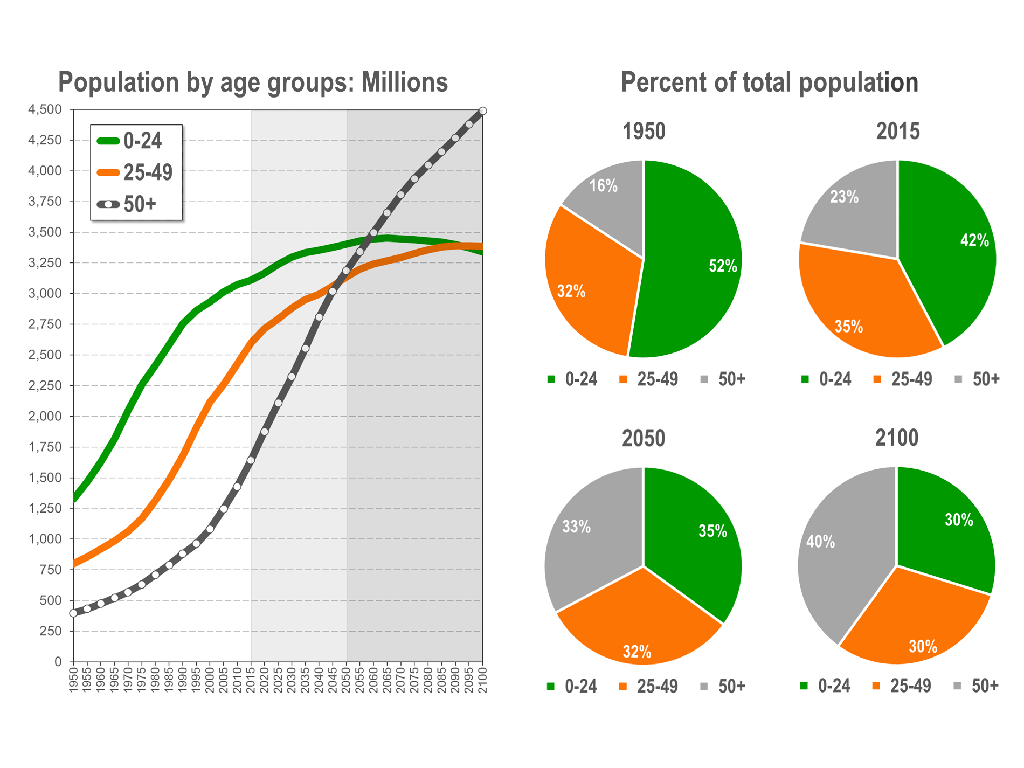
\includegraphics[scale=0.4]{images/human_population.png}
\centering
\caption{Σχηματική απεικόνιση της εξέλιξης του ανθρώπινου πληθυσμού και της ηλικιακής σύνθεσης του. \cite{human_population}}
\label{human_population}
\end{figure}
Είναι σαφές πως η ζήτηση για ποιοτικές υπηρεσίες υγείας έχει αυξηθεί και θα συνεχίσει να αυξάνεται, κυρίως λόγω της αύξησης του πληθυσμού. \cite{Lubitz2003} 
Εξίσου σαφές είναι το γεγονός ότι τα υπάρχοντα συστήματα και μοντέλα παροχής υπηρεσιών υγείας συχνά κρίνονται ανεπαρκή για την κάλυψη αυτής της ζήτησης, εξαιτίας της ανισότητας πρόσβασης σε αυτά, όπως φαίνεται στο γράφημα \ref{insufficient}. 
\begin{figure}[h!]
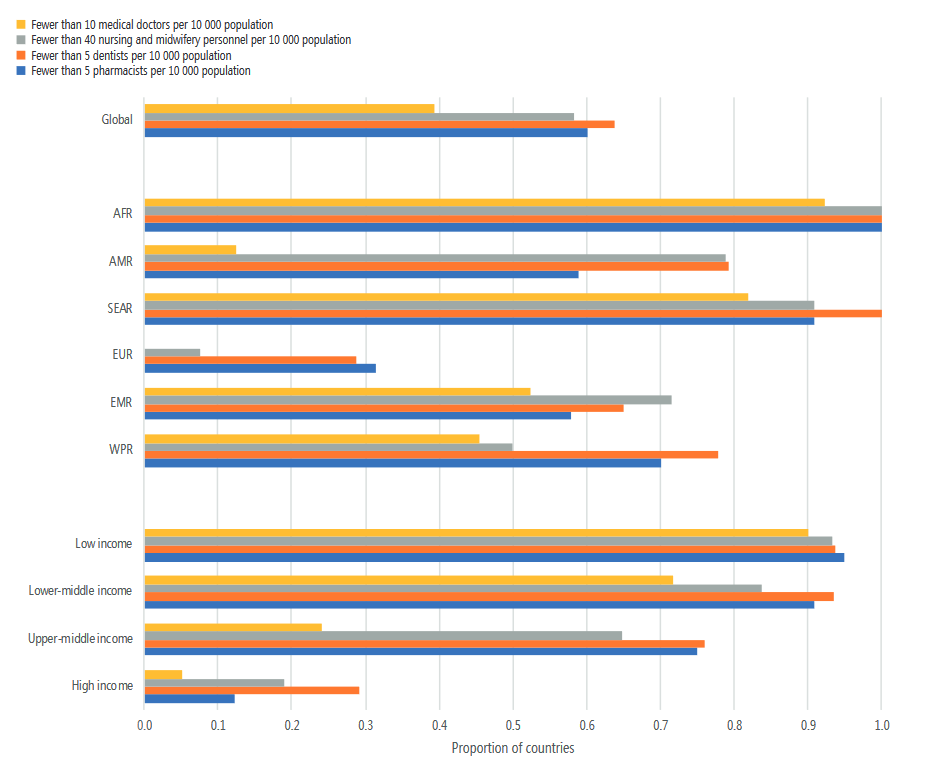
\includegraphics[scale=0.6]{images/who_insufficient.png}
\centering
\caption{Έλλειψη ιατρικού προσωπικού ανάλογα με την ήπειρο και το σχετικό μέσο εισόδημα κάθε χώρας. \cite{WHO}}
\label{insufficient}
\end{figure}
\par

Παρακάτω, αναφέρονται σύντομα ορισμένες από τις μεγαλύτερες προκλήσεις του υπάρχοντος συστήματος υγειονομικής περίθαλψης.
\begin{itemize}
    \item \textbf{Υπηρεσίες υγείας σαν εμπόρευμα} --- Η αντιμετώπιση της παροχής υπηρεσιών υγείας ως εμπόρευμα οδηγεί στην περιθωριοποίηση δαπανηρών αλλά αναγκαίων θεραπειών ή ερευνών.
    \item \textbf{Μειούμενη αναλογία ιατρικού προσωπικού ανά ασθενή} --- Ως συνέχεια του παραπάνω, η μείωση του εξειδικευμένου ιατρικού προσωπικού σε συνδυασμό με την αύξηση του πληθυσμού, οδηγεί σε χαμηλής ποιότητας υπηρεσίες υγείας.
    \item \textbf{Αστικοποίηση} --- Οι σημερινές μητροπόλεις με τα εκατομμύρια πολιτών απαιτούν συνεχείς και μεγάλες επενδύσεις στις υποδομές υγείας, κάτι το οποίο δεν είναι εφικτό ή δεν προτιμάται.
    \item \textbf{Αύξηση του προσδόκιμου ζωής} --- Τέλος, η αύξηση του προσδόκιμου ζωής αυξάνει τον αριθμό των ατόμων που επιζητούν υπηρεσίες υγείας και καθιστά αναγκαία την θεραπεία και διαχείριση χρόνιων παθήσεων.
\end{itemize}
Για την κάλυψη των συγχρόνων κοινωνικών αναγκών υγείας, απαιτείται η επιστράτευση της τεχνολογίας, καθώς και η αλλαγή του μοντέλου υγειονομικής περίθαλψης.
Συγκεκριμένα, απαιτείται να αξιοποιηθούν επικουρικά οι δυνατότητες των νέων τεχνολογιών, όπως και του \en{IoT}, δίχως την περιθωριοποίηση των αναγκών σε ιατρικό προσωπικό και υλικό.
Ταυτόχρονα, και με χρήση των παραπάνω τεχνολογιών, πρέπει να αναδειχθεί η πρόληψη σαν κύριος άξονας της δημόσιας υγείας, δίνοντας ενεργό ρόλο στον πολίτη για την διαχείριση της υγείας του.
\begin{figure}[h!]
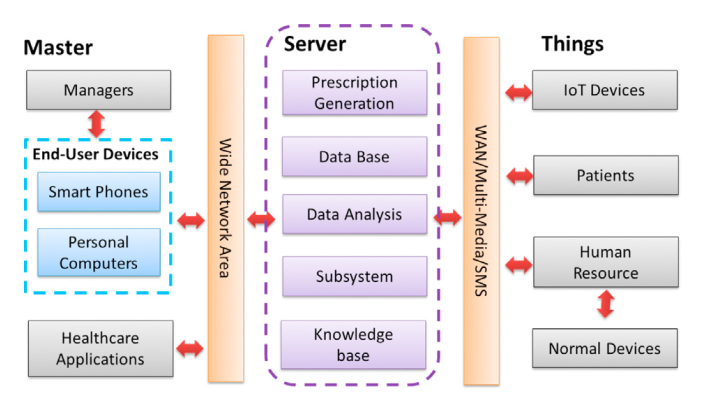
\includegraphics[scale=1]{images/iot_h_example.png}
\centering
\caption{Σχηματική απεικόνιση της αρχιτεκτονικής ενός \en{IoT} συστήματος αποκατάστασης \cite{iot_h_example}}.
\label{iot_h_example}
\end{figure}
\subsection{Λόγοι σύγκλισης}
Οι δυνατότητες των εφαρμογών \en{IoT} μπορούν να καλύψουν ορισμένα από τα προβλήματα που αναφέρθηκαν προηγουμένως. Η δομή των εφαρμογών \en{IoT} μοιάζει με την ιεραρχική δομή ενός συστήματος παροχής υπηρεσιών υγείας, όπως φαίνεται στο Σχήμα \ref{iot_h_example}, όπου βλέπουμε σχηματικά την αρχιτεκτονική ενός συστήματος αποκατάστασης, βασισμένο σε τεχνολογίες \en{IoT}.

Παρακάτω, αναφέρονται ορισμένα από τα πλεονεκτήματα που προσφέρει η χρήση \en{IoT} εφαρμογών στον τομέα της υγείας.
\begin{itemize}
    \item \textbf{Συνεχής και διακριτική καταγραφή των ζωτικών σημείων του ασθενή} ---
    Οι εξελίξεις στην τεχνολογία των βιοαισθητήρων, επιτρέπει την απρόσκοπτη καταγραφή και αποστολή βιοσημάτων από τους ασθενείς, χωρίς να χρειαστεί να αλλάξουν τις καθημερινές τους συνήθειες. Αυτό επιτρέπει την πιο ακριβή και γρήγορη διάγνωση ασθενειών, καθώς και την συλλογή μεγάλου όγκου ιατρικών δεδομένων.
    \item \textbf{Απρόσκοπτη χρήση διάφορων τεχνολογιών} ---
    Η χρήση εφαρμογών \en{IoT} επιτρέπει την χρήση πολλών τεχνολογιών, οι οποίες δεν είχαν εφαρμοστεί πρότερα στον τομέα της υγείας, εξαιτίας της δυσκολίας ενσωμάτωσης τους στις ιατρικές διαδικασίες.
    \item \textbf{Απομακρυσμένη διεπαφή ασθενή και ιατρικού προσωπικού} ---
    Οι εφαρμογές \en{IoT} επιτρέπουν την άμεση, απομακρυσμένη επικοινωνία του ασθενή με κατάλληλο ιατρικό προσωπικό, σε πραγματικό χρόνο. Το προσωπικό αυτό θα έχει άμεση πρόσβαση στα ιατρικό ιστορικό και τα δεδομένα πραγματικού χρόνου του ασθενή.
    \item \textbf{Εξατομικευμένες υπηρεσίες} ---
    Πολλές ασθένειες και παθήσεις δεν εκφράζονται με τον ίδιο τρόπο σε όλους τους ανθρώπους. Η μακρόχρονη συλλογή δεδομένων από έναν ασθενή επιτρέπει την δημιουργία ενός εκτενούς και ακριβούς ιατρικού ιστορικού. Με βάση αυτά τα δεδομένα και την χρήση τεχνικών μηχανικής μάθησης, είναι δυνατή η πρόβλεψη της κατάστασης της υγείας του ασθενή. 
    \item \textbf{Μείωση κόστους} ---
    Η βελτίωση της δυνατότητας πρόβλεψης της υγείας του πολίτη βοηθά την αποτελεσματικότερη διαχείριση του χρόνου του ιατρικού προσωπικού, αλλά και του ιατρικού υλικού.
    \item \textbf{Εύκολη χρήση} ---
    Οι εφαρμογές \en{IoT} στον τομέα της υγείας απευθύνονται και σε άτομα με ειδικές ανάγκες, καθώς και ηλικιωμένους. Οπότε, είναι σχεδιασμένες να χρησιμοποιούνται εύκολα και άμεσα από τους χρήστες τους.
    \item \textbf{Συσσώρευση ιατρικών δεδομένων} ---
    Η συλλογή, επεξεργασία και ανάλυση του τεράστιου πλήθους δεδομένων, που παράγουν οι \en{IoT} εφαρμογές, δίνει νέες δυνατότητες στην ιατρική έρευνα.
\end{itemize}
\subsection{Εφαρμογές}
Η Βιοϊατρική είναι ένας τεράστιος κλάδος, ώστε οι δυνατότητες εφαρμογής των τεχνολογιών του \en{IoT} να μοιάζουν ατέλειωτες, από την απομακρυσμένη παρακολούθηση των ασθενών μέχρι την αντιμετώπιση ασθενειών.
Η χρήση του \en{IoT} περιορίζεται, προς το παρόν, στην τηλεϊατρική και στην καταγραφή και παρακολούθηση κεφαλαίων.
\par
Παρακάτω αναφέρονται οι βασικές εφαρμογές του \en{IoT} στον τομέα της Βιοϊατρικής.
\subsubsection{Περιβάλλοντα Υποβοηθούμενης Διαβίωσης (ΠΥΔ)}
Μια από τις βασικές εφαρμοηές του \en{IoT} είναι η κατασκευή και διαχείριση έξυπνων περιβαλλόντων, τα οποία καθιστούν πιο εύκολη την ζωή των ατόμων που κινούνται μέσα σε αυτά.
Στον τομέα της Βιοϊατρικής, τα άτομα αυτά είναι ασθενείς ή ηλικιωμένοι άνθρωποι, οι οποίοι δεν μπορούν να καλύψουν τις ανάγκες τους χωρίς βοήθεια.
Τα ΠΥΔ αποτελούν βασικό αντικείμενο της διπλωματικής και για αυτό αναλύονται στο κεφάλαιο 2.
\subsubsection{\en{mHealth (mobile Health)}}
Η χρήση του \en{Cloud Computing}, μέσω \en{mobile} και \en{web} εφαρμογών, επιτρέπει την απομακρυσμένη πρόσβαση σε ιατρική πληροφορία.
Ταυτόχρονα, οι ίδιες εφαρμογές επιτρέπουν στο ιατρικό προσωπικό την παροχή οδηγιών και βοήθειας, επικοινωνώντας μέσω \en{video} με τον ασθενή.
Η συγκεντρωμένη ιατρική πληροφορία των ασθενών επιτρέπει στο ιατρικό προσωπικό να παρέχουν πιο άμεση και κατάλληλη θεραπεία για κάθε ασθενή.
\subsubsection{Διαχείριση ιατρικού υλικού}
Η χρήση ετικετών \en{RFID} επιτρέπει την πλήρη διαχείριση του ιατρικού υλικού.
Αρχικά, καθιστά πολύ δυσκολότερη την χάλκευση των ιατρικών προϊόντων, μέσω της μοναδικής ταυτότητας που παρέχει η \en{RFID} ετικέτα.
Στη συνέχεια, κάθε στάδιο της εφοδιαστικής αλυσίδας του προϊόντος καταγράφεται και η πληροφορία αυτή γίνεται διαθέσιμη στον καταναλωτή.
\par
Επίσης, η χρήση εφαρμογών \en{IoT} επιτρέπει την παρακολούθηση της σωστής λειτουργίας κρίσιμων ιατρικών συσκευών, όπως βηματοδότες ή άλλες έμφυτες συσκευές, και ενημερώνει σε πιθανή δυσλειτουργία.
Τέλος, η χρήση ετικετών \en{RFID} επιτρέπει την δημιουργία ενός διαφανούς συστήματος καταγραφής και παρακολούθησης ιατρικών αποβλήτων, σε συνεργασία με τα νοσοκομεία και μεταφορικές εταιρείες. 
\subsubsection{Ψηφιακά νοσοκομεία}
Οι τεχνολογίες που απαρτίζουν το \en{IoT} καθιστούν δυνατή την ψηφιοποίηση και αυτοματοποίηση των διοικητικών διαδικασιών ενός νοσοκομείου, καθώς και την παροχή επαυξημένων δυνατοτήτων στο ιατρικό προσωπικό.
Η σταδιακή εγκαθίδρυση των ηλεκτρονικών μητρώων υγείας, σε συνδυασμό με την χρήση ετικετών \en{RFID} επιτρέπει την άμεση ταυτοποίηση των ασθενών, καθώς και την πρόσβαση στο ιατρικό τους ιστορικό.
Για τον ίδιο λόγο, η διαχείριση ιατρικών επειγόντων περιστατικών γίνεται ευκολότερη, ενώ περαιτέρω βοηθά η διασύνδεση των οργάνων των ασθενοφόρων με το νοσοκομείο.
\par
Η καταγραφή, παρακολούθηση και αξιοποίηση του νοσοκομειακού εξοπλισμού, καθώς και του ιατρικού υλικού, γίνεται ευκολότερη και πιο ακριβής.
Για παράδειγμα, η διαχείριση της αποθήκης φαρμάκων, καθώς και η διανομή τους, μπορεί να γίνει ηλεκτρονικά, αλλά και να αυτοματοποιηθεί.
\par
Επίσης, σημαντικές αλλαγές μπορούν να συμβούν στην διαχείριση των ασθενών και της εμπειρίας τους στο νοσοκομείο.
Αρχικά, η χρήση ετικετών \en{RFID} επιτρέπει στο ιατρικό προσωπικό να έχει περισσότερο έλεγχο στην ροή των ανθρώπων.
Η συνεχής παρακολούθηση των ζωτικών σημείων των ασθενών αποτελεί την βάση ενός έξυπνου συστήματος ειδοποίησης σε περίπτωση ανάγκης.
Ταυτόχρονα, ο ασθενής είναι σε θέση να χειρίζεται το περιβάλλον νοσηλείας του, μέσω τεχνολογιών αναγνώρισης φωνής και \en{mobile} εφαρμογές.
\par
Τέλος, είναι εφικτή η βελτίωση της απόδοσης του ιατρικού προσωπικού, ιδιαίτερα στους τομείς των επειγόντων, της χειρουργικής και της ραδιολογικής.
Η παροχή των απαραίτητων πληροφοριών τους επιτρέπει να πάρουν κρίσιμες αποφάσεις γρηγορότερα και με μεγαλύτερη ακρίβεια.
\subsubsection{Απομακρυσμένη παρακολούθηση ασθενών}
Οι εξελίξεις στον τομέα των βιοαισθητήρων και η καθιέρωση του κλάδου των \en{wearables} καθιστούν δυνατή την απομακρυσμένη παρακολούθηση των ασθενών σε μη κλινικά περιβάλλοντα.
Αυτή περιλαμβάνει την συλλογή σημάτων (βιολογικών και μη) από αισθητήρες, την πιθανή καταγραφή εικόνας και ήχου και την αποστολή τους στο κατάλληλο ιατρικό προσωπικό.
Η πορεία της θεραπείας, οι προτάσεις του ιατρικού προσωπικού και το σύστημα ειδοποιήσεων παρέχονται στον ασθενή, μέσω \en{mobile} εφαρμογών.
\par
Η ένταξη της απομακρυσμένης παρακολούθησης ασθενών στην διαχείριση χρόνιων παθήσεων οδηγεί στην βελτίωση της ποιότητας ζωής των ασθενών.
Τους επιτρέπει να διατηρήσουν την ανεξαρτησία τους και να επιλύουν ευκολότερα επιπλοκές.